\chapter{Wellen in einem Kanal\label{chapter:wellen}}
\lhead{Wellen in einem Kanal}
\begin{refsection}
\chapterauthor{Daniela Meier und Hansruedi Patzen}

\begin{equation}
	y'' + (ax^2+bx+c)y = 0
	\label{wellen:grundgleichung}
\end{equation}

Dieses Kapitel besch"aftigt sich mit Ausbreitung von Wellen in einem 
parabolischen Kanal. Die Ausbreitung wird mittels Analyse der Wellengleichung 
n"aher betrachtet.

\section{Herleitung Ausgangsformel}
In einem ersten Schritt wird erkl"art, wie die 
Gleichung \ref{wellen:grundgleichung} aus der Aufgabenstellung zustandegekommen 
ist.

Die allgemeine Differentialgleichung der Welle lautet (gem"ass 
\cite{wellen:smirnow2}):

\begin{equation*}
	\frac{\partial^2 u}{\partial t^2}
	=
	c^2
	\left(
		\frac{\partial^2 u}{\partial x^2} 
		+ \frac{\partial^2 u}{\partial y^2} 
		+ \frac{\partial^2 u}{\partial z^2}
	\right)
	\label{wellen:allgemeineDGL}
\end{equation*}

Da in der ausgew"ahlten Problemstellung nur eine zweidimensionale Welle 
betrachtet wird, fallen die y- und die z-Koordinate weg. Die Gleichung 
vereinfacht sich dadurch zu:

\begin{equation}
	\frac{\partial^2 u}{\partial t^2}
	=
	c^2
	\left(
		\frac{\partial^2 u}{\partial x^2} 
	\right)
	\label{wellen:allgemeineDGLvereinfacht}
\end{equation}

Somit ist die Funktion $u$ noch abh"angig von der Zeit $t$ und der 
Ortskoordinate 
$x$.

\begin{equation*}
	u = f(x,t)
\end{equation*}

Zur L"osung der vereinfachten Wellengleichung 
\ref{wellen:allgemeineDGLvereinfacht} wird die Theorie des Separationsansatzes 
angewendet. Gem"ass dem kann $u(x, t)$ in ein Produkt zweier Funktionen $X(x)$ 
und $T(t)$ umgewandelt werden.

\begin{equation}
	u (x,t) = X(x) T(t)
	\label{wellen:separierteFunktion}
\end{equation}

Ausgehend von der vereinfachten Grundgleichung der Welle 
\ref{wellen:allgemeineDGLvereinfacht} wird die Funktion 
\ref{wellen:separierteFunktion} auf der linken Seite zweimal partiell nach $t$ 
und auf der rechten Seite zweimal partiell nach $x$ abgeleitet. Daraus 
resultiert:

\begin{equation}
	T''(t) X(x) = c^2 X''(x)T(t)
\end{equation}

Diese Differentialgleichung wird nun durch $T(x)X(x)$ dividiert und somit 
werden die Variablen separiert und ein Term entsteht, welcher nur funktionieren 
kann, wenn beide Seiten der Gleichung konstant sind. 

\begin{equation*}
	\frac{T''(t)}{T(t)}
	=
	c^2 \frac{X''(x)}{X(x)} = \text{konstant} = \lambda
\end{equation*}

Aus dieser Gleichung entstehen nun zwei l"osbare Differentialgleichungen 
zweiter Ordnung.

\begin{equation*}
	T''= \lambda T(t)
\end{equation*}

und

\begin{equation}
	X'' = \frac{\lambda}{c^2}X(x)
	\label{wellen:DGLzweiterOrdnung}
\end{equation}

Bei der betrachteten Problemstellung, wird davon ausgegangen, dass die 
Zeit konstant ist. Aus diesem Grund wird ab hier nur weiter auf die Gleichung 
der Funktion $X(x)$ eingegangen. Wird die Gleichung 
\ref{wellen:DGLzweiterOrdnung} gleich Null gesetzt, ergibt sich:

\begin{equation*}
	X''(x) - \frac{\lambda}{c^2} X(x) = 0
\end{equation*}

Diese Gleichung widerspiegelt die Wellengleichung, die in der Fortsetzung 
betrachtet wird.

Mit dem Faktor $\frac{\lambda}{c^2}$ k"onnen verschiedene 
Geschwindigkeitsprofile betrachtet werden. Hier wird unter anderem auf den 
speziellen Fall eines parabolischen Profils eingegangen. Die zu untersuchende 
Differentialgleichung ergibt sich hiermit zu der am Anfang definierten 
Gleichung \ref{wellen:grundgleichung}, mit den frei w"ahlbaren Variablen 
${a,b,c} \in \mathbb{R}$, sowie den Anfangsbedingungen $y(0) = a_0$ und $y'(0) 
= a_1$.

\section{Potenzreihenl"osung}
Als L"osungsansatz wird der im Kapitel \ref{chapter:potenzreihen} 
kennengelernte Potenzreihenansatz (\ref{potenzreihen:ansatz}) verwendet.

Zuerst wird die Potenzreihe f"ur $y$ aufgestellt und zweimal abgeleitet.

\begin{equation}
	y(x)
	=
	\sum_{k = 0}^{\infty} a_{k}x^k
	=
	a_0 + a_1x + a_2x^2 + a_3x^3 + a_4x^4 + a_5x^5 + a_6x^6 + \dotsb
	\label{wellen:nullteableitung}
\end{equation}

\begin{equation*}
	y'(x)
	=
	\sum_{k=0}^{\infty} a_{k+1}(k+1)x^k
	=
	a_1 + 2a_2x + 3a_3x^2 + 4a_4x^3 + 5a_5x^4 + 6a_6x^5+ \dotsb
\end{equation*}

\begin{equation}
	y''(x)
	=
	\sum_{k = 0}^{\infty} a_{k+2}(k+1)(k+2)x^k
	=
	2a_2 + 3 \mathbin{\cdot} 2a_3x + 4 \mathbin{\cdot} 3a_4x^2 + 5 
	\mathbin{\cdot} 4a_5x^3 + 6 \mathbin{\cdot} 5a_6x^4 + \dotsb
	\label{wellen:zweiteableitung}
\end{equation}

Aus den beiden Gleichungen \ref{wellen:nullteableitung} und 
\ref{wellen:zweiteableitung} kann nun der Koeffizientenvergleich 
\ref{wellen:koeffizietenvergleich} erstellt werden.

\begin{equation}
	\begin{split}
		y''
		&=
		-(ax^2+bx+c)y \\
		2a_2 + 3 \mathbin{\cdot} 2a_3x + 4 \mathbin{\cdot} 3a_4x^2 + \dotsb
		&=
		-(ax^2+bx+c)(a_0 + a_1x + a_2x^2 + a_3x^3 + a_4x^4 + \dotsb) \\
		2a_2 + 3 \mathbin{\cdot} 2a_3x + 4 \mathbin{\cdot} 3a_4x^2 + \dotsb
		&=
		-aa_0x^2-aa_1x^3-aa_2x^4-\dotsb \\
		&\hspace{10pt}
		-ba_0x-ba_1x^2-ba_2^3-ba_3x^4-\dotsb \\
		&\hspace{10pt}
		-ca_0-ca_1x-ca_2x^2-ca_3x^3-ca_4x^4 - \dotsb
	\end{split}
	\label{wellen:koeffizietenvergleich}
\end{equation}

Daraus k"onnen nun die Resultate f"ur die verschiedenen $a_k$ bestimmt werden.

\begin{equation}
	\begin{split}
		a_2
		&=
		-\frac{1}{2}ca_0 \\
		a_3
		&=
		-\frac{1}{3 \cdot 2} (ba_0 + ca_1) \\
		a_4
		&=
		-\frac{1}{4 \cdot 3} (aa_0 + ba_1 + ca_2) \\
		&=
		-\frac{1}{4 \cdot 3} (aa_0 + ba_1 -\frac{1}{2}c^2a_0) \\
		a_5
		&=
		-\frac{1}{5 \cdot 4} (aa_1 + ba_2 + ca_3) \\
		&=
		-\frac{1}{5 \cdot 4} (aa_1 -\frac{1}{2}bca_0 -\frac{1}{3 \cdot 2} 
		c(ba_0 + ca_1)) \\
		&\hspace{5pt}\vdots
	\end{split}
	\label{wellen:aks}
\end{equation}

Hieraus l"asst sich nun eine allgemeine Rekursionsformel 
\ref{wellen:koeffizientengleichung} f"ur die verschiedenen $a_k$ herauslesen. 
Es gilt: $k \in \mathbb{N}$ und	$a_{k < 0} = 0$

\begin{equation}
	a_{k+2} = -\frac{1}{(k+2)(k+1)} (aa_{k-2}+ba_{k-1}+ca_k)
	\label{wellen:koeffizientengleichung}
\end{equation}

Nun kann man die L"osungsgleichung \ref{wellen:ygleichung} f"ur $y(x)$ 
aufstellen.

\begin{equation}
	y(x) = a_0 + a_1x 
	-\sum_{k=0}^{\infty}\frac{1}{(k+2)(k+1)}(aa_{k-2}+ba_{k-1}+ca_k)x^{k+2}
	\label{wellen:ygleichung}
\end{equation}

Um das Programmieren dieser Formel zu vereinfachen, formt man sie am besten von 
$a_{k+2}$ nach $a_k$ um. Damit erh"alt man die Gleichung 
\ref{wellen:koeffizientengleichungak}.
Bei der neuen L"osungsgleichung f"ur $y(x)$ \ref{wellen:ygleichungak} muss nun 
aber $k \in \mathbb{N} \backslash \{0, 1\}$ gelten.

\begin{equation}
	a_{k} = -\frac{1}{k(k-1)} (aa_{k-4}+ba_{k-3}+ca_{k-2})
	\label{wellen:koeffizientengleichungak}
\end{equation}

\begin{equation}
	y(x) = a_0 + a_1x 
	-\sum_{k=2}^{\infty}\frac{1}{k(k-1)}(aa_{k-4}+ba_{k-3}+ca_{k-2})x^k
	\label{wellen:ygleichungak}
\end{equation}

\section{Erkenntnisse bei der Variation von \texorpdfstring{$k_{max}$}{kmax}}

Es wird davon ausgegangen, dass sich mit der Variation von $k_{max}$ bei der 
Welle keine grossen Ver"anderungen einstellen. Die Werte werden immer ab einem 
gewissen Punkt ins Positive oder Negative explodieren, da das $x^k$ irgendwann 
dominiert. Mit $k_{max}$ wird die Anzahl der Summanden bezeichnet, die f"ur die 
Berechnung der Potenzreihe verwendet werden. 

\begin{equation*}
y(x) = a_0 + a_1x 
-\sum_{k=2}^{k_{max}}\frac{1}{k(k-1)}(aa_{k-4}+ba_{k-3}+ca_{k-2})x^k
\end{equation*}

Es werden die Startbedingungen gem"ass den Gleichungen 
\ref{wellen:Startbedingungen1} festgelegt.

\begin{equation}
	\begin{split}
		a_0 &= 1\\
		a_1 &= 0\\
		a &= 1\\
		b &= 0\\
		c &= -1
	\end{split}
	\label{wellen:Startbedingungen1}
\end{equation}

Auf folgenden Grafiken wird veranschaulicht, was mit der Welle passiert, wenn 
das $k_{max}$ jeweils um 30 vergr"ossert wird. Es wird dann "uberpr"uft, ob 
sich die Behauptung der kleinen Ver"anderungen als wahr herausstellt.

\begin{center}
	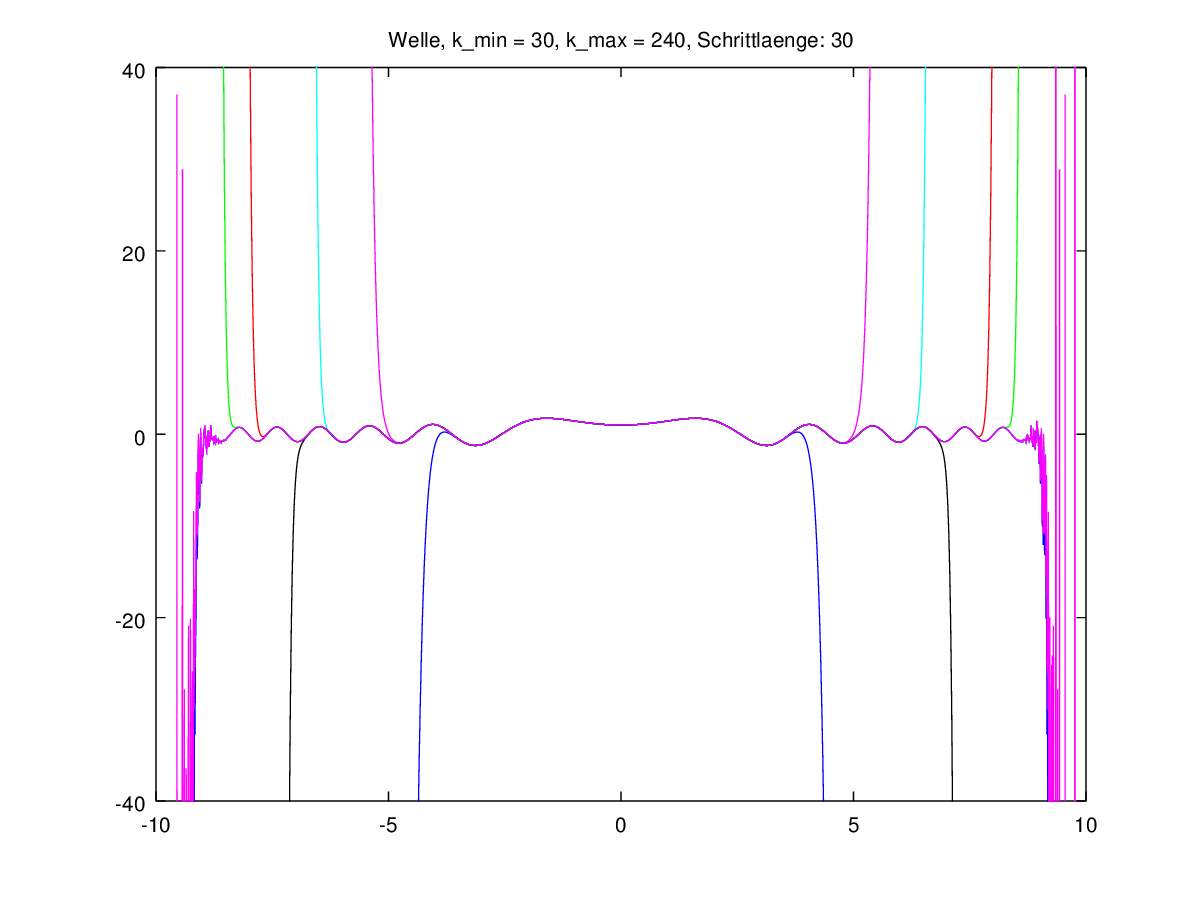
\includegraphics[scale=0.69]{./wellen/octave/images/kmax/krangewaveeven.png}
\end{center}

Die Behauptung, dass der Wert irgendwann explodiert, ist, wie ersichtlich, 
wahr. Der Punkt wo die Werte gegen $\infty$ gehen verschiebt sich immer mehr 
nach rechts, zu gr"osseren $x$-Werten. Dies wird dadurch erkl"art, dass es 
immer l"anger geht, bis der $x^k$-Term dominiert. Je mehr der $k_{max}$-Wert 
gesteigert wird, umso besser wird die Approximation an die Welle. Ab einer 
gewissen Gr"osse von $k_{max}$ kann das Programm die Werte nicht mehr genau 
bestimmen, was die unregelm"assigen Ausschl"age erkl"art.

Aufgrund dieser Messungen wird $x$ f"ur die weiteren Berechnungen auf $x \in 
[-8;8]$ und $k_{max}$ auf 180 beschr"ankt, damit die $y$-Werte nicht 
explodieren und keine unkontrollierten Messwerte entstehen.

Mit den in diesem Kapitel festgelegten Startbedingungen und Einschr"ankungen 
ergibt dies folgende Grafik:
\begin{center}
	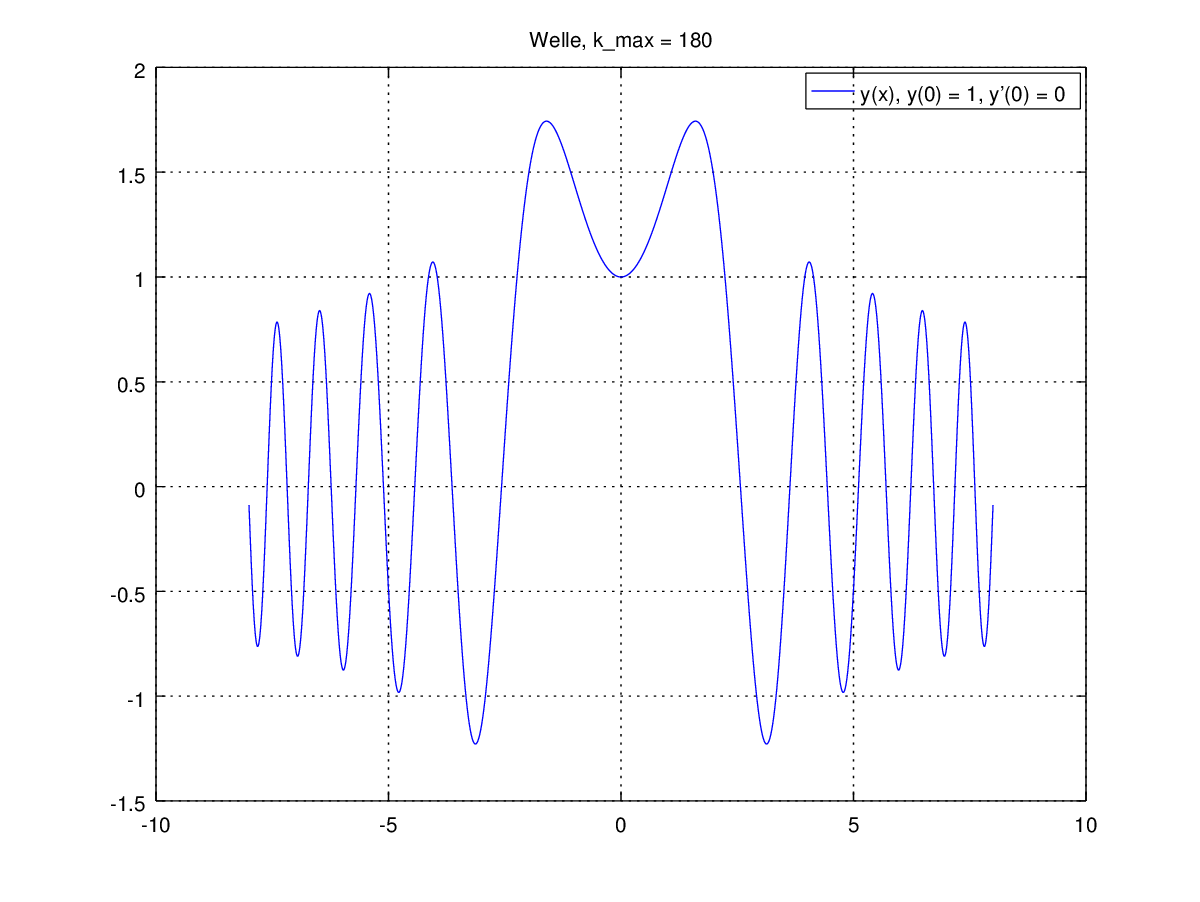
\includegraphics[scale=0.69]{./wellen/octave/images/kmax/ak180-88wave.png}
\end{center}

\section{Erkenntnisse bei der Variation von \texorpdfstring{$a$}{a}, 
\texorpdfstring{$b$}{b} und \texorpdfstring{$c$}{c}}

Die Anfangsbedingungen $a_0$ und $a_1$ k"onnen beliebig festgelegt werden. Da 
sich die Wellen im betrachteten Fall um den Entwicklungspunkt $x_0=0$ bewegen, 
beschreibt das $a_0$ den y-Achsenabschnitt und das $a_1$ die Steigung im Punkt 
$y(0)$. Die gew"ahlten Werte von $a_0$ und $a_1$ sind jeweils in der Grafik 
ersichtlich.

\subsection{Eliminierung von $a$ und $b$}
\label{wellen:Eliminierungab}

Zu Beginn wird das vorgegebene, parabelf"ormige Geschwindigkeitsprofil 
n"aherungsweise in eine Konstante umgewandelt indem $a$ verschwindend klein 
gew"ahlt wird und $b$ gleich $0$ gesetzt wird. Die beiden Variablen werden also 
eliminiert und folgende Differentialgleichung wird betrachtet:

\begin{equation}
	y''+ cy = 0.
	\label{wellen:lineareDGL}
\end{equation}


F"ur positive Werte von c kann die L"osung dieser Gleichung 
\ref{wellen:lineareDGL} mit dem charakteristischen Polynom bestimmt werden. 
Die L"osungen des charakteristischen Polynoms

\begin{equation}
	p(\lambda) = [(\lambda+\mu)^2+\omega^2] =0
	\label{wellen:charakteristischesPolynom}
\end{equation}

sind

\begin{equation}
	\begin{split}
	y_1 &= C_1e^{-\mu x}\cos(\omega x) \\
	y_1 &= C_2e^{-\mu x}\sin(\omega x).
	\end{split}
	\label{wellen:lsgcharakteristischesPolynom}
\end{equation}

Das zur Gleichung \ref{wellen:lineareDGL} geh"orende charakteristische Polynom 
ist gem"ass \ref{wellen:charakteristischesPolynom}

\begin{equation*}
	p(\lambda) = [\lambda^2 + c] =0.
\end{equation*}

Somit folgt die allgemeine L"osung der Differentialgleichung 
\ref{wellen:lineareDGL} gem"ass \ref{wellen:lsgcharakteristischesPolynom}

\begin{equation}
	y(x) = C_1 \cos(\sqrt{c}x) + C_2 \sin(\sqrt{c}x)
	\label{wellen:LsglineareDGL}
\end{equation}

Um die Konstanten $C_1$ und $C_2$ zu bestimmen m"ussen die Anfangsbedingungen 
$a_0$ und $a_1$ bekannt sein. Um die Abh"angigkeit aufzuzeigen, muss zuerst die 
erste Ableitung der L"osung \ref{wellen:LsglineareDGL} aufgestellt werden.

\begin{equation}
	y'(x)=-C_1 \sqrt{c} \sin(\sqrt{c}x) + C_2 \sqrt{c} \cos(\sqrt{c}x)
\end{equation}

Der Wert bei $y(0)$ ist definiert als $a_0$ und die Steigung am Punkt $y'(0)$ 
ist das $a_1$. Setzt man $x=0$ in die L"osungsgleichung 
\ref{wellen:LsglineareDGL} ein, k"onnen $C_1$ und $C_2$ bestimmt werden.

\begin{equation}
	\begin{split}
		y(0) = C_1 = a_0 &\Leftrightarrow C_1 = a_0 \\
		y'(0) = C_2 \sqrt{c} = a_1 &\Leftrightarrow C_2 = \frac{a_1}{\sqrt{c}}
	\end{split}
	\label{wellen:KonstantenC1C2}
\end{equation}

Setzt man diese Konstanten \ref{wellen:KonstantenC1C2} in die L"osungsgleichung 
\ref{wellen:LsglineareDGL} 
ein, ergibt sich die Gleichung, die sich mit den Startangaben, die definiert 
werden, f"ur positive $c$-Werte berechnen l"asst.

\begin{equation}
	y(x) = a_0 \cos(\sqrt{c}x) + \frac{a_1}{\sqrt{c}} \sin(\sqrt{c}x)
	\label{wellen:LSGleichung}
\end{equation}

In den folgenden zwei Grafiken werden die zwei Grundfunktionen von ``reinem''
Sinus (erste Grafik) und Cosinus (zweite Grafik) aufgezeigt. Daf"ur muss 
entweder $a_0$ oder $a_1$ gleich Null gesetzt werden.

\noindent
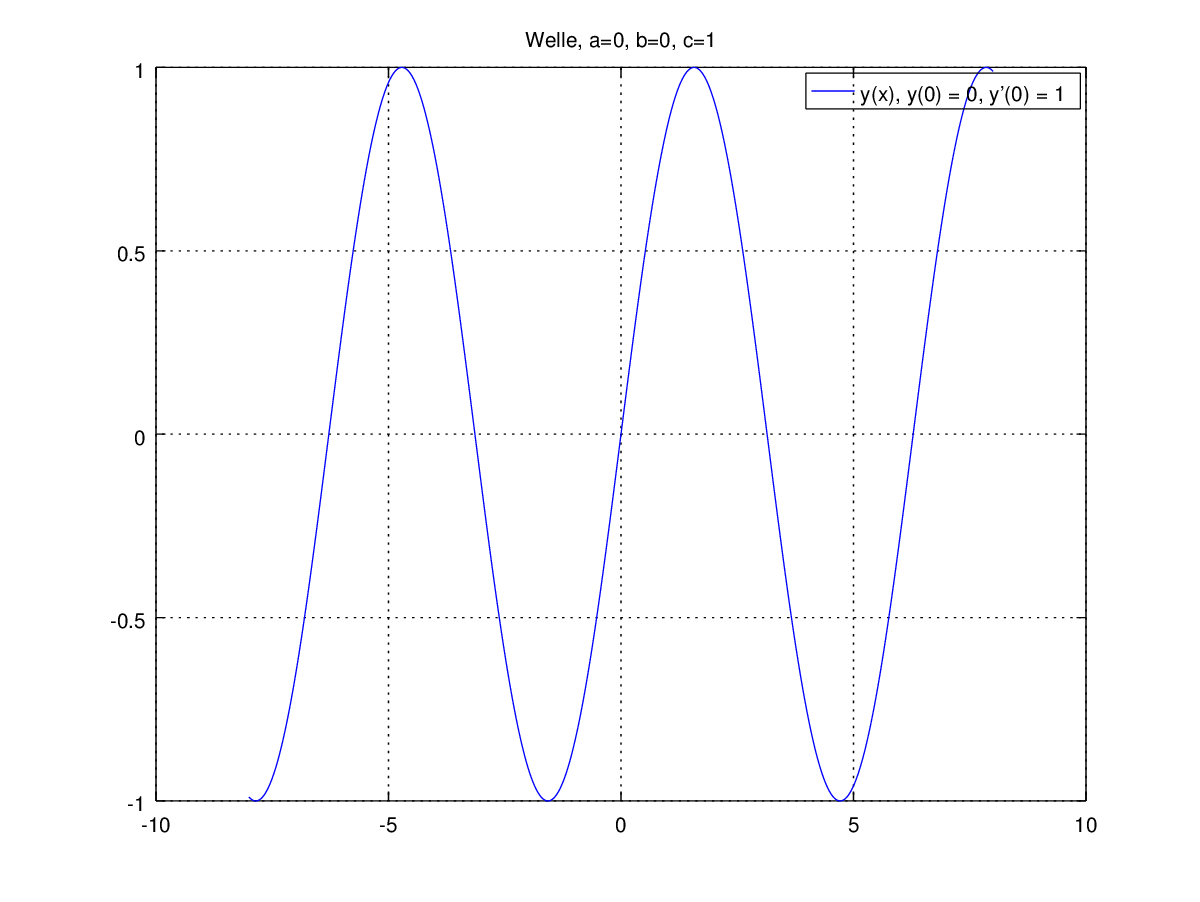
\includegraphics[scale=0.35]{./wellen/octave/images/grundfunktionen/sin.png}
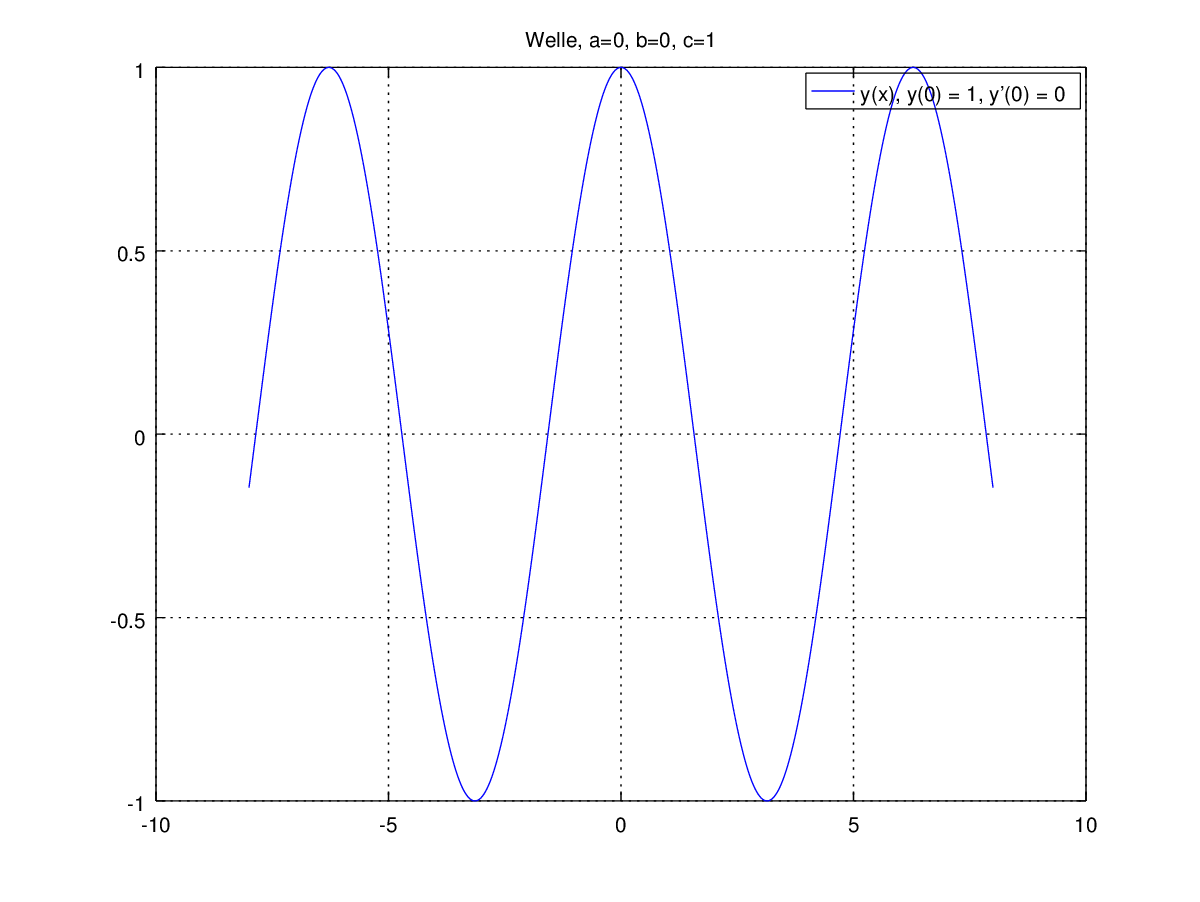
\includegraphics[scale=0.35]{./wellen/octave/images/grundfunktionen/cos.png}

F"ur negative Werte von c kann die L"osungsgleichung \ref{wellen:LSGleichung} 
zwar auch verwendet werden, es entstehen aber imagin"are Faktoren durch die 
negativen Wurzelwerten. Die imagin"are Einheit $i$ ist definiert als

\begin{equation}
	i = \sqrt{-1}.
	\label{wellen:imaginaereEinheit}
\end{equation}

Wird dieser Wurzelwert \ref{wellen:imaginaereEinheit} bei jedem negativen Wert 
von $c$ ausgeklammert, ergibt sich die L"osungsgleichung.

\begin{equation}
	\begin{split}
	y(x) &= a_0 \cos(i\sqrt{|c|}x) + \frac{a_1}{i\sqrt{|c|}}\sin(i\sqrt{|c|}x) 
	\\
	\Leftrightarrow
	y(x) &= a_0 \cos(i\sqrt{|c|}x) - i\frac{a_1}{\sqrt{|c|}}\sin(i\sqrt{|c|}x)
	\end{split}	
	\label{wellen:LSGnegcWerte}
\end{equation}

Die Definitionen vom Sinus Hyperbolicus und Cosinus Hyperbolicus lauten:

\begin{equation*}
	\begin{split}
	\sinh(x) &= \frac{1}{2} (e^x - e^{-x}) = -i \sin(ix)\\
	\cosh(x) &= \frac{1}{2} (e^x + e^{-x}) = \cos (ix)
	\end{split}
\end{equation*}

Werden die Definitionen mit der L"osungsformel verglichen, ist ersichtlich, 
dass es sich je nach Wahl von $a_0$ und $a_1$ um eine der beiden hyperbolischen 
Funktionen handelt. Die L"osungsgleichung ergibt sich also zu

\begin{equation}
	y(x) = a_0 \cosh(\sqrt{|c|}x) + \frac{a_1}{\sqrt{|c|}}\sinh(\sqrt{|c|}x)
	\label{wellen:LSGhyperbolFunktion}
\end{equation}

In den folgenden zwei Grafiken wird zuerst der ``reine'' Sinus Hyperbolicus und 
als zweites der ``reine'' Cosinus Hyperbolicus dargestellt.

\noindent
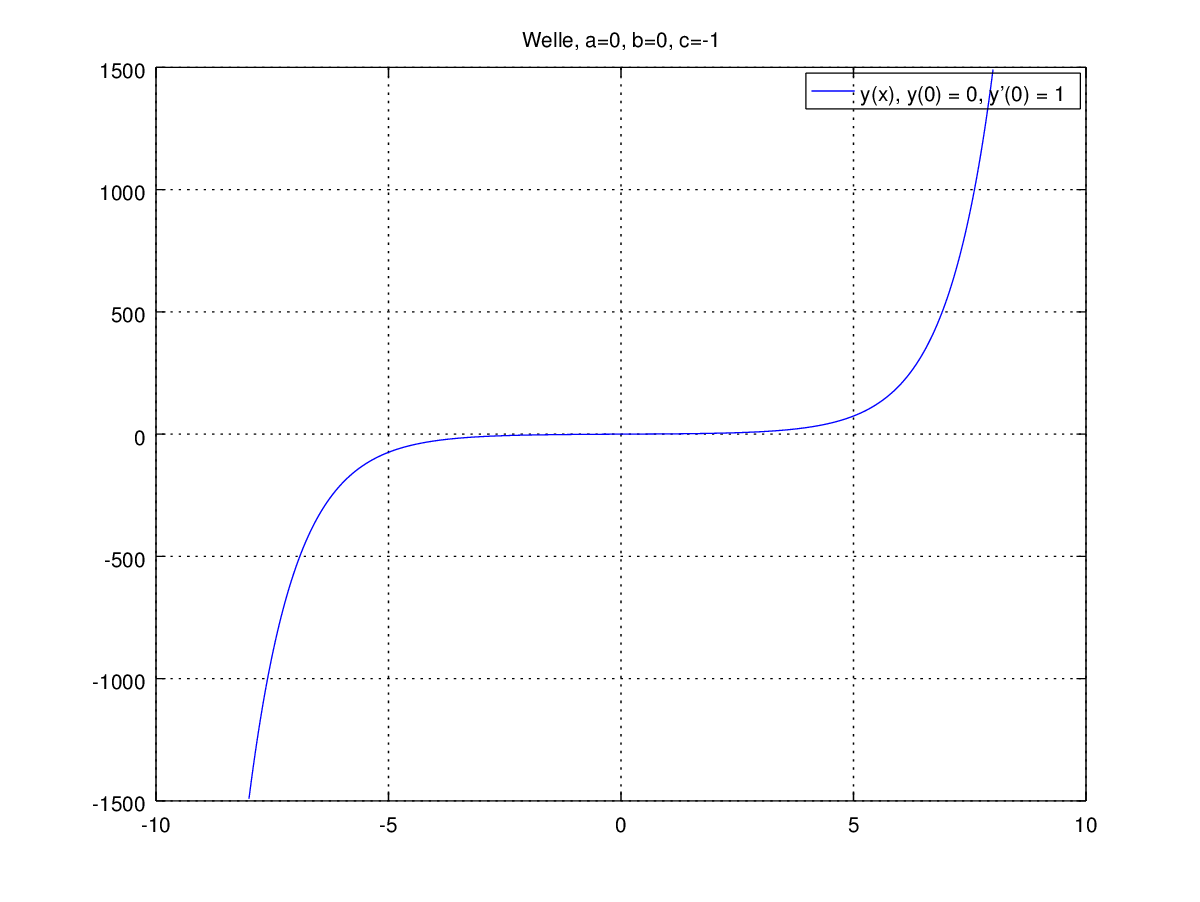
\includegraphics[scale=0.35]{./wellen/octave/images/grundfunktionen/sinh.png}
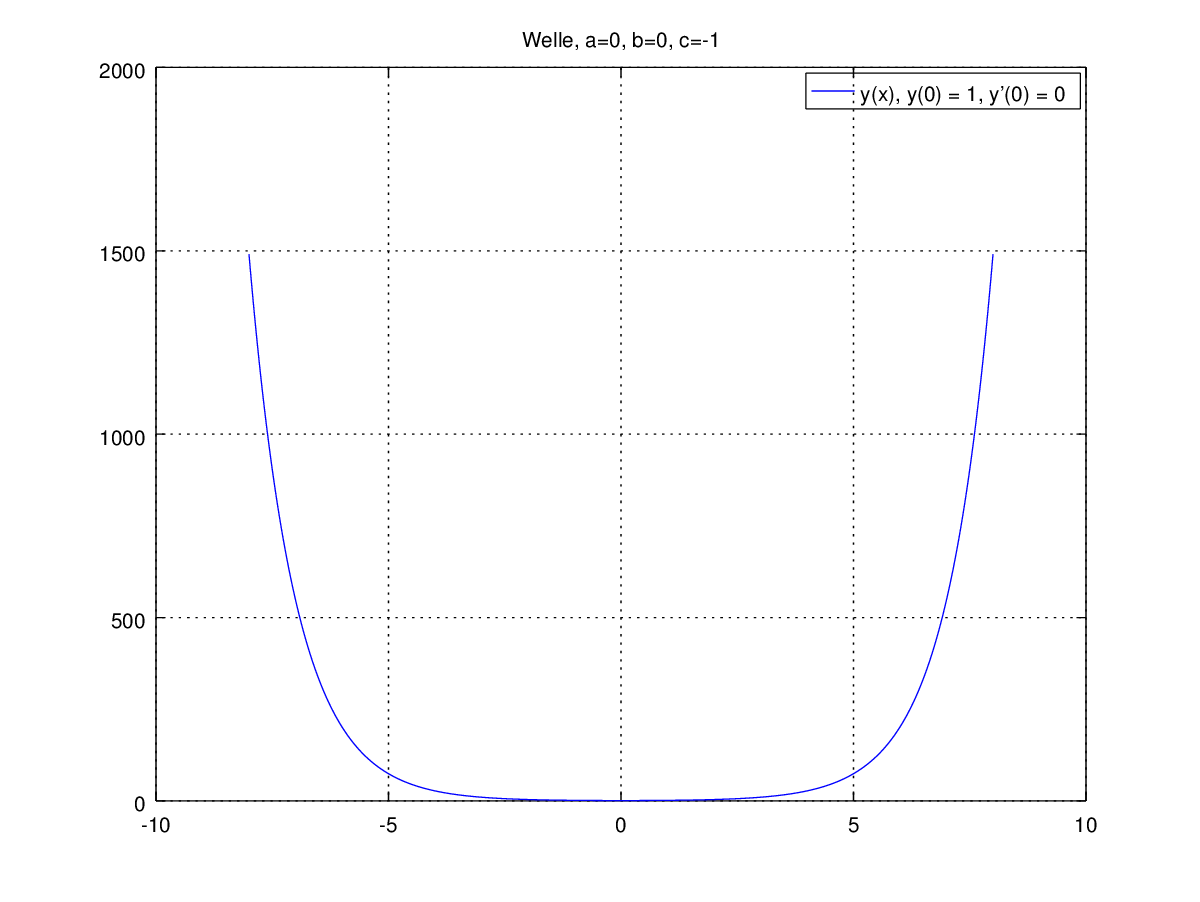
\includegraphics[scale=0.35]{./wellen/octave/images/grundfunktionen/cosh.png}

\subsection{Variation von $b$}

Als Zweites werden die Variablen $a$, $c$ und die Anfangsbedingungen 
festgehalten und nur das $b$ ver"andert. Um aufzuzeigen, was sich dabei 
ver"andert, braucht es nur die Parabelgleichung.

\begin{equation*}
	y(x) = ax^2 + bx + c
\end{equation*}

BILD VERSCH. PARABELN

Der Faktor $b$ bezweckt n"amlich, wie man in der Grafik sieht, in der Parabel 
nur eine Verschiebung in Richtung der $x$-Achse. Diese Verschiebung bedeutet in 
der betrachteten Problemstellung nur, dass sich die Schnittpunkte mit der 
$x$-Achse verschieben. Was dies bedeutet wird in einem sp"ateren Abschnitt 
erkl"art. Was aber aus der Variation mit $b$ herausgeht ist, dass wir die 
dadurch ver"anderten Eigenschaften auch mit der Variation von $c$ oder von 
$a_0$ aufzeigen k"onnen. Aus diesem Grund wird die Variabel $b$ in Fortsetzung 
immer gleich 0 gesetzt und damit vernachl"assigt. 

Die neue zu betrachtende Differentialgleichung ergibt sich damit zu:

\begin{equation} 
	y'' + (ax^2 +c)y = 0
	\label{wellen:DGLzubetrachten}
\end{equation}

\subsection{Variation von $c$}
\label{wellen:Variationc}

Als N"achstes wird untersucht, welche Auswirkungen die Variation vom 
Koeffizienten $c$ hat, wenn $a$ vorhanden ist und nicht gegen 0 geht aber 
trotzdem festgehalten wird. $a$ wird in der folgenden Betrachtung gleich 1 
gesetzt.

Der Koeffizient $c$ beschreibt den Schnittpunkt der Parabel mit der $y$-Achse 
und somit die Verschiebung in $y$-Richtung. Diese Verschiebung kann nicht, wie 
die Verschiebung in Richtung der $x$-Achse mit dem Koeffizienten $b$, 
vernachl"assigt werden. Grund daf"ur ist, dass die Wellenform vom Schnittpunkt 
der Parabel mit der $x$-Achse abh"angt. 

\noindent
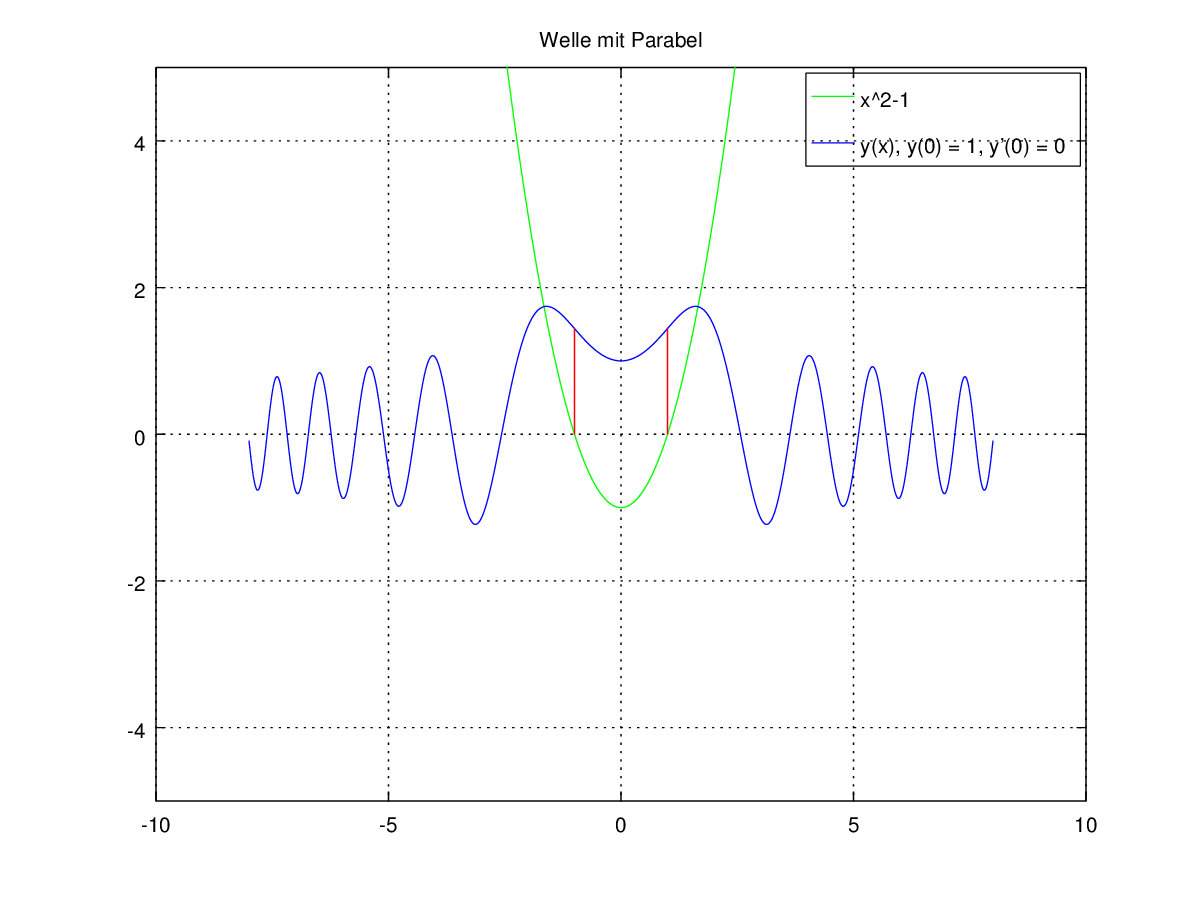
\includegraphics[scale=0.35]{./wellen/octave/images/variationc/cneg1.png}
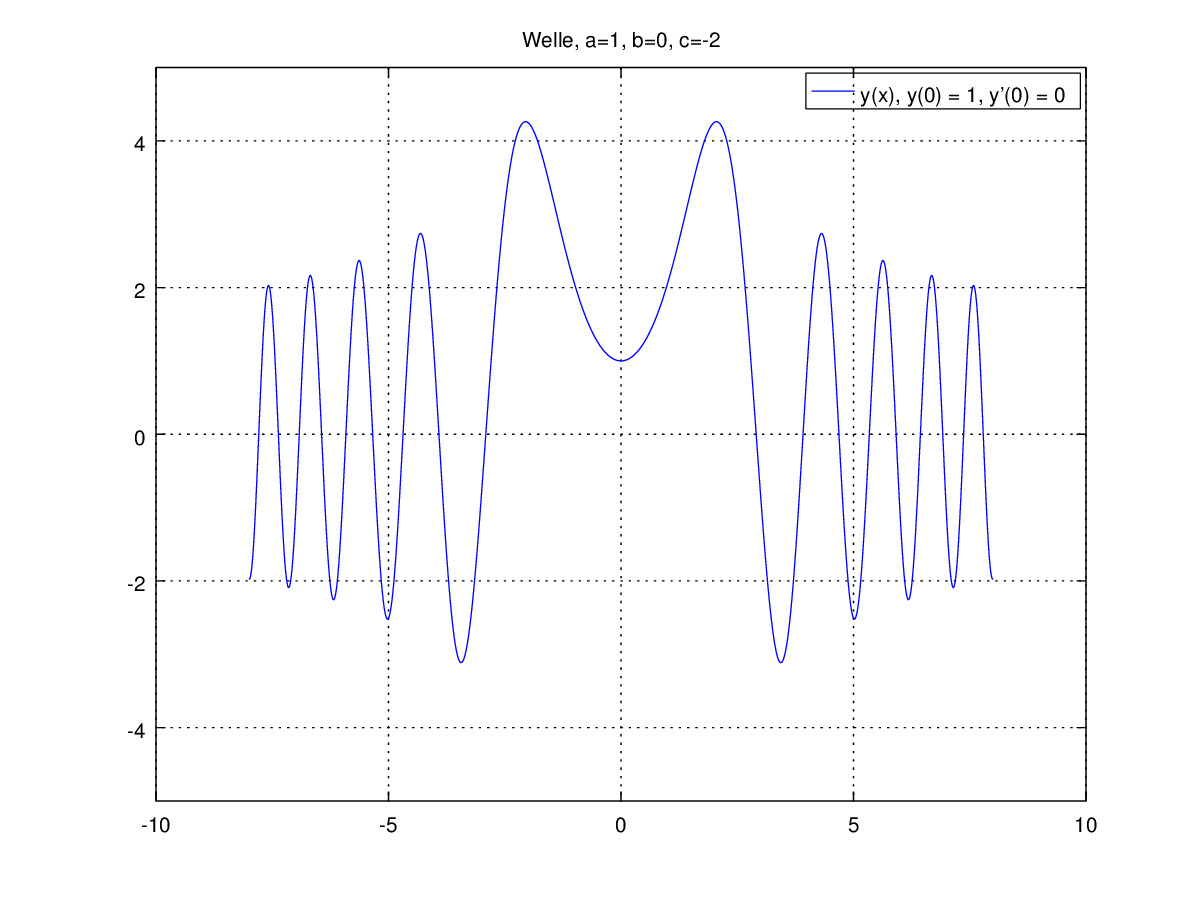
\includegraphics[scale=0.35]{./wellen/octave/images/variationc/cneg2.png}

In den zwei Grafiken werden die 
Parabeln mit zwei unterschiedlichen $y$-Achsenabst"anden und deren aus der 
Differentialgleichung \ref{wellen:DGLzubetrachten} entstehende Welle gezeigt. 
Es wird deutlich, dass es nicht die gleiche Welle gibt und dass sich beim 
Schnittpunkt der Parabel mit der $x$-Achse eine "Anderung einstellt. Dieses 
Ph"anomen wird im n"achsten Kapitel \ref{wellen:DiskussionWellenform} erkl"art. 

\subsection{Variation von $a$}
\label{wellen:Variationa}

Zum Schluss wird der Koeffizient $a$ variiert, was zur Folge hat, dass die 
Parabel schl"anker oder enger wird. Dadurch verschiebt sich auch der 
Schnittpunkt der Parabel mit der $x$-Achse und somit auch der Umschlagspunkt, 
der im Kapitel \ref{wellen:Variationc} schon ersichtlich war. 

...

\section{Diskussion der Wellenform}
\label{wellen:DiskussionWellenform}

Wie schon in den vorhergehenden Kapiteln ersichtlich war, wechselt die Welle 
ihre Form im ``Umschlagspunkt'', welcher die Schnittpunkte der Parabel mit der 
$x$-Achse bezeichnet.


Grunds"atzlich gibt sechs untschiedliche F"alle wie die Parabel liegen kann:
\begin{itemize}
	\item Der Schnittpunkt der Parabel mit der $y$-Achse ist im negativen 
	Bereich und die Parabel nach oben ge"offnet
	\item Der Schnittpunkt der Parabel mit der $y$-Achse ist im positiven 
	Bereich und die Parabel ist nach oben ge"offnet
	\item Der Schnittpunkt der Parabel mit der $y$-Achse liegt im Nullpunkt und 
	die Parabel ist nach oben ge"offnet
	\item Der Schnittpunkt der Parabel mit der $y$-Achse ist im negativen 
	Bereich und die Parabel nach unten ge"offnet
	\item Der Schnittpunkt der Parabel mit der $y$-Achse ist im positiven 
	Bereich und die Parabel nach unten ge"offnet
	\item Der Schnittpunkt der Parabel mit der $y$-Achse liegt im Nullpunkt und 
	die Parabel ist nach unten ge"offnet
\end{itemize}

Zu Beginn wird der erste Fall betrachtet, welcher beispielsweise die Parabel 
auf der Grafik im Kapitel \ref{wellen:Variationc} beschreibt. Diese Parabel hat 
zwei Schnittpunkte mit der $x$-Achse und der Scheitelpunkt liegt im negativen 
$y$-Bereich. Dies bedeutet, dass alle L"osungen der Parabel von $x=0$ bis zum 
Schnittpunkt der Parabel mit der $x$-Achse negativ sind. 

Wenn nun in der Differentialgleichung f"ur die Parabel ein beliebiger negativer 
Wert eingesetzt wird, resultiert dieselbe Gleichung \ref{wellen:LSGnegcWerte} 
wie im Kapitel \ref{wellen:Eliminierungab}. Durch das, dass die Parabel durch 
einen Wert ersetzt wird, ist die Aufgabenstellung die Gleiche, wie wenn man $a$ 
und $b$ eliminieren und f"ur $c$ einen negativen Wert einsetzen w"urde. In 
diesem Bereich entsteht demzufolge gem"ass Gleichung 
\ref{wellen:LSGhyperbolFunktion} eine hyperbolische Funktion. Welche von den 
zwei hyperbolischen Funktionen entsteht, l"asst sich mit verschiedenen 
Anfangsbedingungen $a_0$ und $a_1$ bestimmen wie man in den folgenden Grafiken 
sieht.

GRAFIK SINH COSH

Beim Schnittpunkt der Parabel mit der $x$-Achse "andert sich das Vorzeichen der 
L"osung der Parabel und es entsteht nicht die Gleichung 
\ref{wellen:LSGnegcWerte} wie oben, sondern die Gleichung 
\ref{wellen:lineareDGL}, welche f"ur positive $c$-Werte aufgestellt wurde. 

Daraus wird ersichtlich, dass sich ab diesem Punkt eine L"osung einstellt, 
welche aus einer "Uberlagerung von $\sin$ und $\cos$ ist. Daraus entsteht die 
regelm"assige, kontinuierliche Schwingung. 


Bei all den anderen F"allen kann das Gleiche beobachtet werden. Bei der Parabel 
die nach oben ge"offnet ist, passiert genau das Umgekehrte. Im Innenbereich der 
Parabel entsteht eine Schwingung und sobald die Parabel die $x$-Achse schneidet 
wandelt sich die Schwingung in eine hyperbolische Funktion um. 4

Bei den Parabeln, die die $x$-Achse im Nullpunkt ber"uhren entsteht nur eine 
Schwingung, respektive nur eine hyperbolische Funktion, je nach Wert von a, 
welcher angibt, ob die Parabel nach oben oder nach unten ge"offnet ist. 
Dasselbe geschieht auch, wenn die Parabel die $x$-Achse gar nicht schneidet. 







\printbibliography[heading=subbibliography]
\end{refsection}